\documentclass{article}
\usepackage{amsmath}
\usepackage{enumerate}
\usepackage{graphicx}
\usepackage{hyperref}
\usepackage{fancyvrb}
\usepackage[margin=0.5in]{geometry}
\usepackage{cleveref}
\usepackage{xcolor}
\usepackage{listings}
\RecustomVerbatimCommand{\VerbatimInput}{VerbatimInput}%
{fontsize=\footnotesize,
	frame=lines,  % top and bottom rule only
}

\newcommand{\quotes}[1]{``#1''}

\begin{document}
	\title{PIV Remote Computing Guide}

	\author{Travis Burrows}
	\maketitle
	
	\tableofcontents
	\newpage
	
	\section{Abstract}
	This is a guide to the process of remotely computing PIV on the Georgia Tech PACE cluster, which includes generating the DaVis processing script on your local machine, installing DaVis on your PACE account, transferring data to the PACE server, submitting a job for PIV processing, and finally downloading the results.

	\section{Log into PACE via SSH}
	SSH, or Secure Shell, is the method used to log into your PACE account via command line.  This will be required to submit PIV jobs to the PACE computing nodes.
	
	\subsection{Software}
	If you are using Windows, you will have to install software to be able to SSH into PACE.  KiTTY and PuTTY are both good options.  Download KiTTY from \url{https://www.fosshub.com/KiTTY.html}.  Both portable and installer versions are available.
	
	\subsection{Connection Settings}
	Once you have launched one of these programs, you will need to enter in a url.  The proper url for SSH is \nolinkurl{login-s.pace.gatech.edu} .  Click to save to save it for the future, and then Start or Open to initiate the connection.  You will be prompted for your username and password.  In addition, if you get asked about an unknown host key, press yes to accept the key.  

	\begin{figure}[h!]
		\centering
		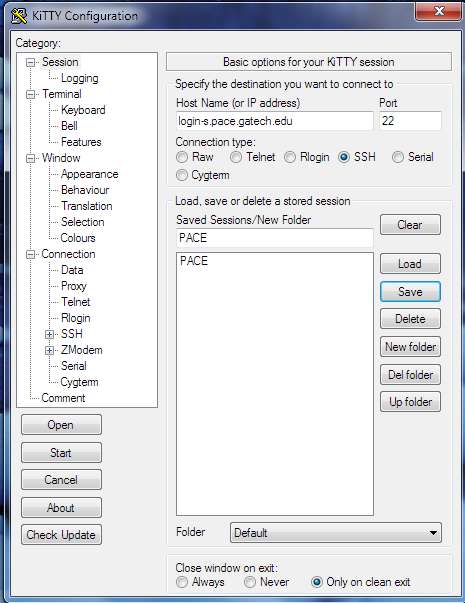
\includegraphics[width=3in]{./kitty.png} 
		\caption{KiTTY Interface}
	\end{figure}
	
	\subsection{SSH Commands}
	Congratulations!  You've SSH'd into PACE!  Now the possibilities are limitless- as long as you know the commands (you are in a linux system).  To change directories, use the command \nolinkurl{cd}.  To list the files in a folder, use \nolinkurl{ls}.  To exit, you can simply type \nolinkurl{exit}, or exit out of the window like any other.

	\section{Transferring files to and from PACE}
	This section will cover how to transfer files to and from PACE.  There are a couple of options available, which are using SFTP (SSH File Transfer Protocol) or using the Globus software.  Once it is properly set up, Globus will be the faster and more direct way to get files to PACE.  Since it is not set up yet, the procedure is not yet documented.

	\subsection{SFTP}
	
	\subsubsection{Software}
	\label{software}
	If you don't already have a favorite file transfer program, I would recommend FileZilla.  Download and install the Filezilla Client software from \url{https://filezilla-project.org}.  This works like any typical FTP file transfer program.  If you are using Windows and want to mount PACE as if it is another drive on your computer, see \Cref{webdrive}.
	
	\subsubsection{Connection Settings}
	\label{connection}
	PACE has special servers for data transfer, which are different from the servers used for SSH.  For file transfer, use \nolinkurl{iw-dm-4.pace.gatech.edu}.  Your GT username and password will work to authenticate and get you connected.  If you have not yet been given access to PACE, you will find out when you fail to connect.  In FileZilla, go to File $\rightarrow$ Site Manager $\rightarrow$ New Site to create this new connection.  Select Protocal as SFTP, enter the above url into Host, and enter your GT username and password into the appropriate locations, if you would like auto-login.  Save the site entry and click connect.
	
	\begin{figure}[h!]
    	\centering
    	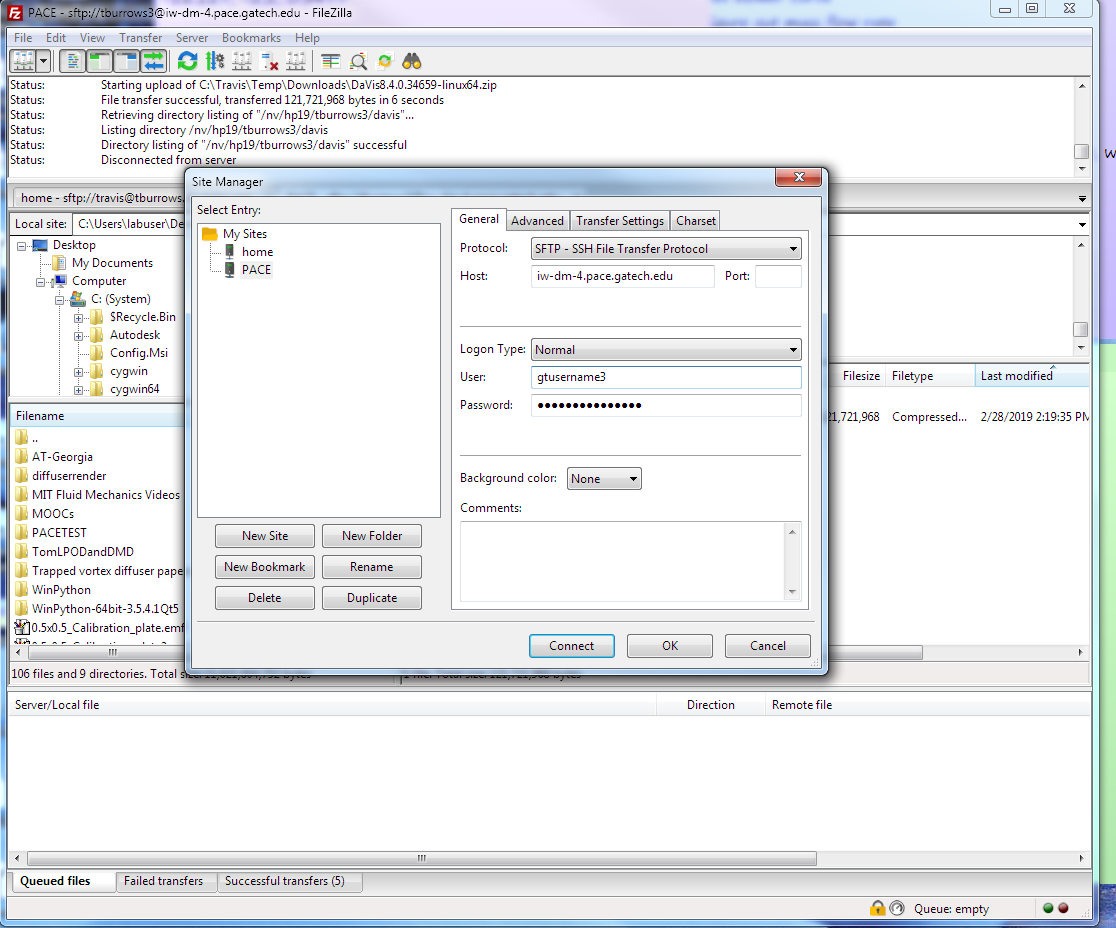
\includegraphics[width=6in]{./filezilla.png} 
    	\caption{FileZilla Interface}
	\end{figure}
	
	\subsubsection{Transferring Files}
	After connecting, you should see a list of folders populate on the right half of the window.  This is the PACE folder structure, while on the left is the local machine.  To upload files or folders from the local machine to PACE, you can drag-and-drop, or right-click and select upload.  This will upload into currently selected folder on the remote computer.  You can download files from the remote to local computer by selecting download or dragging files in the opposite direction.
	
	\subsubsection{WebDrive}
	\label{webdrive}
	WebDrive is software that can mount an SFTP connection as a Windows drive letter.  This will not take advantage of a 10G connection, but does make accessing the files convenient.  Get the software from \url{http://software.oit.gatech.edu}.  Log in, and find WebDrive under FTP/VPN software.  Install it using the provided license and enter the same SFTP connection details as described in the \Cref{software}.  Note that this is a connection to only your personal PACE folder and could cause confusion if it is a shared machine.
	
	\subsection{Globus}
	Globus is the preferred method to transfer files to and from PACE.  Before your local machine can be used for transfers, Globus software must be installed, so your computer is registered as an Endpoint.
	
	\subsubsection{Installing Globus on a Local Machine}
    \begin{enumerate}
        \item Check if your compueter has Globus Connect Personal installed in your programs.  If so, make sure it is currently running, and note what the Endpoint Name is, by hovering over the icon in the taskbar.
	    \item Navigate to \url{https://www.globus.org} and log in with the Glezer shared account
	    \item Click Endpoints $\rightarrow$ Administered by You.  If your PC is shown here and the status is Ready, then you are ready to transfer files.  If your computer does not have Globus Connect Personal installed, or it is installed but does not show up here, you will have to uninstall and install again.
	    \item To install Globus Connect Personal, click Endpoints, and Create a personal Endpoint, which is in the top right corner of the webpage.  Choose a name for the PC that the lab will understand, click Generate Setup Key, and dowload the installer.
	    \item Run the installer on your local PC, and enter the setup key when asked.
	    \item When you are asked about editing shared locations on your PC, go in and edit them.  Add all locations on the PC that you might want to transfer files to and from.  Only these locations will be available for transfer.
	\end{enumerate}
	
	\subsubsection{Transferring files with Globus}
	Once your local PC has Globus Connect Personal installed, follow these steps to make transfers.
	\begin{enumerate}
	    \item Select your local PC for a transfer by clicking File Manager $\rightarrow$ Collection Search $\rightarrow$ Your Collections $\rightarrow$ Your PC
	    \item Click Transfer or Sync to... $\rightarrow$ Search $\rightarrow$ PACE Internal
	    \item Log in to PACE Internal with your regular GT credentials (not Glezer shared)
	    \item On the left side (local PC), navigate to the folder or files you would like to send or receive
	    \item On the right side (PACE Internal), navigate to the folders or files you would like to send or receive
	    \item Select all files/folders you would like to transfer
	    \item If you want to only transfer new files, or update only files that have been changed, you can find advanced settings under Transfer \& Sync Options.
	    \item If you would like to transfer Right $\rightarrow$ Left, click the start button on the left that points right.  If you want to transfer Right $\leftarrow$ Left, click the start button on the right side that points left.
	    \item Find the status of your transfers in the pane called Activity.  You can also cancel transfers here.
	    
	    
	\end{enumerate}
	
	\subsection{PACE Storage Folders}
	When you connect to PACE you will by default be in your PACE home directory.  The path of this folder is something like \nolinkurl{/nv/hp19/yourusername}.  This folder, the home folder, has a limit of 5 GB of storage, and is backed up daily.  Therefore, it should not be used for PIV processing.  The subfolder called \nolinkurl{scratch} is designed to be a temporary data storage location, and has a limit of 7 TB.  Files older than 60 days are automatically deleted, and are not backed up.  The folder called \nolinkurl{data} has a limit of 2 million files/folders, is daily backed up, and can be used for longer-term storage.  Therefore, the safest place to conduct PIV processing is in the \nolinkurl{data} folder.  Note that \nolinkurl{data} and \nolinkurl{scratch} are actually shortcuts to other drives.  They can be reached by the path \nolinkurl{~/scratch}, or the actual path, which can be found in FileZilla upon navigating into one of these folder.	
	
	\section{Installing DaVis on PACE}
	\label{installdavis}
	\begin{enumerate}
		\item Obtain the file \texttt{DaVis8-linux64.zip} from \texttt{P:/Shared/PACE PIV Tutorial} or the latest from the LaVision website.
		\item Using a file transfer program, make a folder in your home directory called \texttt{davis}.  Then, transfer the zip file into that new folder.
		\item SSH into your PACE account.  By default you should be in your home directory.  Change directories into the folder that contains the davis zip file. (\texttt{cd davis}).
		\item Type the command \texttt{unzip DaVis8-linux64.zip} to unzip the contents into the current folder.
		\item The linux DaVis will only work with a slight modification - follow these steps to rename one of the folders in the DaVis installation.  Rename the \texttt{linux64} folder to\texttt{ linux64.old} (\texttt{mv linux64 linux64.old }).  Now, rename the folder \texttt{linux64-centos69} to \texttt{linux64} (\texttt{mv linux64-centos69 linux64}).
		\item Now, setup DaVis in cluster mode by running \texttt{./davis-setup.sh cluster} .  This initializes the installation into cluster mode.  You should receive this message: \\ \texttt{Starting DaVis to setup cluster configuration...\\Done. The script generated by the DaVis master can now be processed.}
		\item Another test to make sure that DaVis is correctly configured is to run \texttt{./davis-start.sh}.  This should give a fairly long output,  listing the node's specifications, as well as DaVis available packages.  It should be clear that the program shut down on its own and didn't throw any errors. 
		\item Finally, set your davis installation to be read only.  This helps prevent processors from changing it while others are using it.  Do this by running the following command: \texttt{chmod -R a-w $\sim$/davis} .  Your DaVis install is now ready for processing!  Proceed to creating a processing script from your local DaVis.
		
		
	\end{enumerate}
	
	\section{DaVis Processing Script}
	This step is the process of generating a script on your local machine, which tells the remote DaVis installation where the data is that will be processed, and what processing settings will be used.  This script is required for PACE remote PIV processing.
	
	\subsection{Requirements}
	The feature in DaVis that we are using is called Cluster Script Processing.  This feature must be enabled in your DaVis license, which you can check by going to DaVis $\rightarrow$ Help $\rightarrow$ About.  If it is not enabled, note your dongle number from the About screen, and contact Callum Gray at LaVision for a replacement license file that contains this feature.
	
	\subsection{Script Generation}
	
	\begin{enumerate}
			\item 	The button for script generation is found in the Processing dialog.  Pick a data set (image set) that you want to process, and open the Processing dialog for it. 
			
			\item 	Before clicking the button, choose what operations you would like the remote computers to perform.  It is recommended to first run Test Processing on the settings you want to use, to make sure that the results look good.  A caveat is that only certain operations are supported by Cluster Script Processing.  This is because of how the operations are implemented by LaVision - only certain ones can be parallelized on multiple machines.  PIV and vector postprocessing are supported, but many are not, like time subtraction and vector averaging.  These do not take much processing power anyway.  To use PACE, you will have to process on your own machine the other operations manually, which means doing any time-subtraction or others beforehand, and averaging after the instantaneous vector fields are downloaded from PACE.\footnote{Another option is to assign different nodes whole data sets, in which case the image pairs are not distributed to different machines.  This function has not been explored or documented as of yet.}
			
			\item	Once your processing operations are chosen, click \quotes{Create Processing Script}.  This will warn you if you have operations selected that are not distributable.  A new window pops up, with a lot of options.  The top half of the dialog is auto-filled, and cannot be modified.  The bottom half needs to be changed.  \quotes{Script Folder} is the folder on the local machine that you want to save this script.  Pick or make a folder dedicated for these scripts.  \quotes{Linux local script path} is the path on the PACE machine that you will place this script.  \quotes{Linux local program path} is the path on the PACE machine where you have installed the linux version of DaVis.  \quotes{Linux local project path} is the path on the PACE machine where you have copied your project folder from the the local machine where the data was recorded.  \quotes{Generate script} is the name of the script itself.  \quotes{File list} will be filled by DaVis, and \quotes{Distribution system} should say OpenMPI.
			
			If you have not yet installed DaVis on your PACE account, or chosen a PACE folder for your PIV processing, come back here after you have done so so that you know what paths need to be entered.
			
			\begin{figure}[h!]
				\centering
				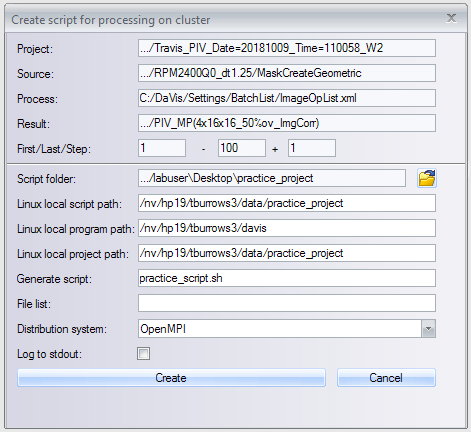
\includegraphics[width=5in]{./cluster_script_processing.png} 
				\caption{Create Processing Script popup dialog}
			\end{figure}
	\end{enumerate}

	\section{Submitting the job to the PACE Queue}
	\subsection{Prerequisite: Transfer PIV Files to PACE}
	Before submitting your PIV job, all the files need to be in the correct places on PACE, and these paths need to match those in the DaVis cluster processing script.  The project path specified in the script must contain the same files that your local project folder has, including the xml file that corresponds to the project folder.  It does not need to contain other data sets that you are not currently processing.  See the example zip file and the practice exercise in \Cref{PracticeExercise} for an example of where the files should be placed.
	
	\subsection{Using PACE computing cluster}
	This section explains how to get PACE to run the DaVis script that has been generated.  It is assumed that at this point, the script and PIV data files have been placed on PACE, at the correct location, and that you are SSH'd into PACE.  There are two ways to compute on PACE - interactive mode, and batch mode.  Batch mode is more convenient for bulk processing PIV.
	
	\subsubsection{Interactive mode}
	In interactive mode, the user requests a certain amount of computing resources, for a certain amount of time.  This request is placed via a command.  Once this command is ran, it submits the request and waits until it is available.  When it is available, access to the computing node is returned, and you will find yourself logged into it, automatically.  Once you are here, you can run whatever you would like, until the time is over, when you will be kicked off.  The following is the command:
	\\ \\
	\texttt{qsub -I -q prometheus -l nodes=1:ppn=8,walltime=10:00:00,pmem=4gb}
	\\  \\
	This requests for computing resources on the cluster called Prometheus, for one node that has 8 cores per node, for 10 hours, and 4 GB per core (32 GB total) .  The choice of cluster and resource specifications will be discussed in \Cref{jobresources}.  This way of interacting with PACE can be useful for debugging or other scenarios, but not really for PIV processing.  Once you have figured out how to properly process, using batch mode is more convenient.
	
	\subsubsection{Batch mode}
	Instead of returning the computing cluster access directly to the user, this method takes an input text file that explains what the cluster should do, and submits this in the queue as a job.  Once it reaches the front of the queue, the job runs in the background, and can email the user when the job is complete.  This text file is called  a PBS script, and an example of how it is structured is shown below.  A pound sign \texttt{\#} followed by a space is considered a comment, while \texttt{\#PBS} is considered a command for the queuing system.
	
	\VerbatimInput{pivjob.txt}
	
	The first section of the text file describes to the job scheduler what resources to use, and settings for output and email notification.  The second section describes what the cluster should do, which in this case is to load the required modules for MPI parallelism, and then run in parallel the DaVis processing script.  The command to submit the job to the queue is simple: \texttt{qsub pivjob.txt} .
	
	\subsubsection{Choosing job resource parameters}
	\label{jobresources}
	\begin{enumerate}
		\item Cluster - As a student in ME, you have access to the ME cluster \quotes{prometheus}.  In addition, there are shared queues which contain other clusters as well.  An illustration of this concept is shown below.  In prometheus, you have the highest priority compared to other users, while in other shared queues that contain prometheus and other clusters, your queue priority goes down.  However, in the shared queues, there are more computers available.  To check what queues you have access to, you can run \texttt{pace-whoami} when logged into PACE.  It will list the queues, corresponding priorities, and maximum wall times you are allowed to use on those queues.  Shared queues you have access to probably include prometforce-6 and iw-shared-6,.  In addition, you can check how many nodes each of these queues has by running \texttt{pace-check-queue queuename}.
		\begin{figure}[h!]
			\centering
			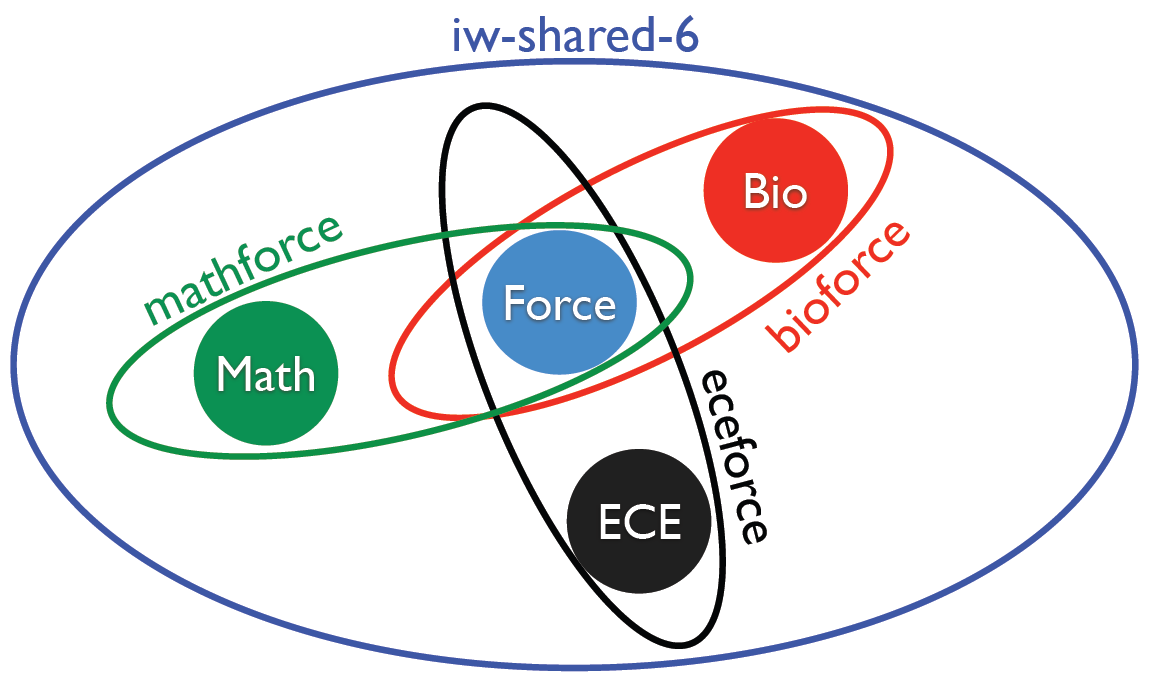
\includegraphics[width=4in]{./clusters.png} 
			\caption{Concept of shared queues}
		\end{figure}
	
		\item Number of nodes - The more nodes you choose, the faster DaVis will process the PIV, but it may take longer for your requested job to start running, depending on how many nodes are currently in use.  In addition, it is not clear exactly how much faster the PIV will process with more nodes.  Conduct a study!  Note that communication between cores on a single node is much faster than between nodes, so increasing the number of cores per node would have a greater effect on performance.
		
		\VerbatimInput{pacecheckqueueprometheus.txt}
		
		\item Processors per node - This requests a certain number of cores on each node to be used.  However, different computing queues only have certain types of computers available, which only have so many cores per node.  You can browse the computers on a queue by running \texttt{pace-check-queue queuename}, as I have on prometheus, shown above.  This shows that prometheus only has 24 and 28 core nodes (in the tasks/np column).  Therefore, if you request 24 or less nodes, any single node could run the job, when it has that many nodes available.  If more than 24 are requested, only the nodes with 28 nodes can complete the job.  But if more than 28 cores are requested, the job will never be completed.  Experiment to see what results in the best computation performance.

		\item Memory per core - This governs how much memory is allocated for your job, per core used.  For planar and stereo PIV, 4 GB should be fine.  If you're curious, run a study and see if more makes a difference.
		
		\item Wall time - This is the amount of time you would like to reserve the resources.  Be conservative but not extremely so, because the longer the wall time, the longer it will take for your job to get started.
	\end{enumerate}

    \section{Practice Exercise}
    \label{PracticeExercise}
    The original practice exercise has been modified in order to circumvent some Davis 8.4 bugs that prevent that technique from working.  Many of the steps in this are exactly the same (1-12)
    \begin{enumerate}
        \item Install FileZilla and KiTTY as shown in \Cref{software}.
    	\item SSH into PACE and run \texttt{pace-whoami} to see what clusters you have access to, and your corresponding priority.
    	\item Run \texttt{pace-check-queue queuename} for each queue you have access to. Check out the number of cores each node has.
    	\item Run \texttt{pace-quota} to check data storage restrictions on your home, data, and scratch drives.
    	\item Run \texttt{pwd} to find out what the absolute path of your home directory is.
    	\item Install Davis as described in \Cref {installdavis}, and note the absolute path of your Davis installation that should look something like \texttt{/nv/hp19/tburrows3/davis}
    	\item Now, find a PIV computer with the cluster script processing enabled, and unzip the \quotes{practice\_project.zip} included archive onto the desktop.
    	\item Open DaVis and set the Project directory to \texttt{Desktop/practice\_project}.  Navigate to \texttt{ Travis\_PIV\_Date=20181009} \texttt{\_Time=110058\_W2 / RPM2400Q\_dt1.25 / MaskCreateGeometric}.  Now, open the processing dialog and load the processing xml file included in the practice project folder.  This has PIV and PIV postprocessing loaded.  \textbf{NOTE: Check and make sure the first item on the processing list is not disabled.  If it is, there will or could be an error in the processing.  This is a bug in DaVis.}
    	\item Press the Create Processing Script button and enter the same values as the included screenshot, except change the  absolute path to yours.  Your home directory might not be in \texttt{/nv/hp19/}.  Make sure to set the script directory to the practice project folder as the screenshot does.  You can tell this step has completed by finding the script in the practice folder, along with a new directory with the same name as the script.  In addition, placeholder folders have been made for the PIV and postprocessing results, within the PIV project folder.
    	\item Using FileZilla, transfer this whole folder \texttt{practice\_project} to your data folder on PACE.  This folder should contain the cluster script, the new cluster script folder, the PIV folder with corresponding xml and exp files, and the python function \texttt{batch-submit.py}.
    	\item Before submitting the job, you need to modify permissions of the practice script .sh file to make it executable.  To back to your SSH terminal and run \texttt{chmod +x practice\_script.sh}.  Your working directory must be the folder which contains this script.
    	\item Test the script \texttt{practice\_script.sh} to see if it works properly before submitting the job.  To know if it works, first open up the script (\texttt{nano practice\_script.sh}) and delete the flag on the last line of the file that disables output, which is \texttt{-stdoff}.  With this removed, DaVis will tell you what is happening.  Now, save the file by pressing ctrl+x, y, then enter.  Now, type \texttt{./practice\_script.sh}.  You should start seeing messages from DaVis, eventually indicating that it is processing.  Note that you are currently processing on the PACE head note, not a compute node.  So once you have proved to yourself that it works, cancel it by pressing ctrl+c.  Insert the \texttt{-stdoff} flag back into the file.  An example of what this script looks like is shown below:
    	
    	\newpage
    	\VerbatimInput{practice_script.sh}
    	
    	\item Instead of directly submitting this script, it will be submitted through the python program \texttt{batch-submit.py}.  This method submits a single job, which requests for all of the computing resources desired to process the set of images.  It is the same as the original method in \Cref{OldExercise}, but the python function makes it more convenient.
    	
    	\item Before you can run the python file, you will have to load Python 3, by running \texttt{module load python/3.6}
    	
    	\item The python file acts as a function which requires arguments, including script name, number of processors, and walltime in hours.  There are other optional parameters, including queue, memory and email notifications.  The default queue is iw-shared-6 and the default memory is 4GB, so it is not strictly necessary to provide this information.  Just run \texttt{python batch-submit.py} for a detailed description of how to use the function. \textbf{For this exercise, try 20 processors and 1 hour of walltime.  This will split up the image set into 20 jobs of 5 images each with an hour to finish, which is way more than needed.}
    	
    	\item Run the function in your terminal on \texttt{practice\_script.sh} with 20 processors for an hour by typing \texttt{python batch-submit.py practice\_script.sh 20 1}
    	
    	\item After running the function, you should see printed output showing that the jobs have been submitted to the queue.
    	
    	\item Check the status of your job by running \texttt{qsub -u username}.  If you want to delete the submitted job, type \texttt{qdel ********}.
    	
    	\item To tell if your jobs have completed, you can run \texttt{qsub -u username}, which will give your job the status of C (Complete) when the whole array of jobs is finished.  
    	
    	\item When the jobs have completed, go back into FileZilla/Globus and download the vector files that were computed.  You are done!  Load them in your local DaVis to visualize them and do additional processing.
	\end{enumerate}
    
    \section{Tips and Tricks}
    \begin{itemize}
        \item To check how many vector files have been created so far, in terminal change directories (\texttt{cd}) to the folder that will contain the vc7 files.  Then type \texttt{ls | wc -l} to check the current number of files.  To continuously monitor the number of files, type \texttt{watch "ls | wc -l"}
        \item You might find that all your images didn't process.  Unfortunately, Davis is not free of bugs.  I have found that sometimes when I submit a job that contains PIV and Vector Postprocessing functions, it fails.  But when I only submit PIV computing functions, it works.  In this situation, you would have to do the postprocessing locally.
    \end{itemize}
    \subsection{Custom Linux shortcuts}
    Here is the procedure to create your own custom commands, to make things more convenient.
    \begin{enumerate}
        \item Create a directory in your PACE home directory ($\sim$) called scripts
        \item Edit a hidden file in your home directory called \texttt{.bashrc} with the command \texttt{nano .bashrc}
        \item Add the following text to the end of the file: \texttt{PATH=$\sim$/scripts:\$PATH}
        \item Save the \texttt{.bashrc} file and run the command \texttt{source .bashrc}
        \item Go to $\sim$/scripts and make a file called \texttt{qme} with the following contents, where you enter your username instead of gtusername
        \VerbatimInput{qme}
        \item Move the \texttt{batch-submit.py} file to \texttt{$\sim$/scripts}
        \item Make a file called \texttt{submit} with the following contents:
        \VerbatimInput{submit}
        \item Now, you can be in any directory and run the python batch submit file with the command \texttt{submit}.  Also, you can just type \texttt{qme} to check your queue rather than the longer command \texttt{qstat -u gtusername}
    \end{enumerate}
    
	\section{Appendix}
	\subsection{Old Practice Exercise}
	\label{OldExercise}
	This is the first practice exercise written for using Davis with PACE.  It turns out there are some bugs in Davis, preventing this method from always working.  Instead, see \Cref{PracticeExercise}.
	
	\begin{enumerate}
		\item Install FileZilla and KiTTY as shown above.
		\item SSH into PACE and run \texttt{pace-whoami} to see what clusters you have access to, and your corresponding priority.
		\item Run \texttt{pace-check-queue queuename} for each queue you have access to. Check out the number of cores each node has.
		\item Run \texttt{pace-quota} to check data storage restrictions on your home, data, and scratch drives.
		\item Run \texttt{pwd} to find out what the absolute path of your home directory is.
		\item Now, find a PIV computer with the cluster script processing enabled, and unzip the \quotes{practice\_project.zip} included archive onto the desktop.
		\item Open DaVis and set the Project directory to \texttt{Desktop/practice\_project}.  Navigate to \texttt{ Travis\_PIV\_Date=20181009} \texttt{\_Time=110058\_W2 / RPM2400Q\_dt1.25 / MaskCreateGeometric}.  Now, open the processing dialog and load the processing xml file included in the practice project folder.  This has PIV and PIV postprocessing loaded.  \textbf{NOTE: Check and make sure the first item on the processing list is not disabled.  If it is, there will or could be an error in the processing.  This is a bug in DaVis.}
		\item Press the Create Processing Script button and enter the same values as the included screenshot, except change the username to yours.  If other parts of your home directory path are different too, change that (\texttt{/nv/hp19/}).  Make sure to set the script directory to the practice project folder as the screenshot does.  You can tell this step has completed by finding the script in the practice folder, along with a new directory with the same name as the script.  In addition, placeholder folders have been made for the PIV and postprocessing results, within the PIV project folder.
		\item Exit out of DaVis, and open the pivjob.txt file.  This is the PBS script you will submit to PACE.  Replace the username placeholders with your username.  The rest of the paths should be valid if you have followed the steps correctly thus far.
		\item Using FileZilla, transfer this whole folder \texttt{practice\_project} to your data folder on PACE.
		\item Before submitting the job, a couple modifications to the files need to be made.  First, you need to modify permissions of the practice script .sh file to make it executable.  Run \texttt{chmod +x practice\_script.sh}.  In addition, the PBS script file is in a windows text file format, but needs to be in a unix format.  Run \texttt{dos2unix pivjob.txt}.  This should tell you it successfully converted the file.
		\item If you would like, you can test the script \texttt{practice\_script.sh} to see if it works properly before submitting the job.  To know if it works, first open up the script (\texttt{nano practice\_script.sh}) and delete the flag on the last line of the file that disables output, which is \texttt{-stdoff}.  With this removed, DaVis will tell you what is happening.  Now, save the file by pressing ctrl+x, y, then enter.  Now, type \texttt{./practice\_script.sh}.  You should start seeing messages from DaVis, eventually indicating that it is processing.  Note that you are currently processing on the PACE head note, not a compute node.  So once you have proved to yourself that it works, cancel it by pressing ctrl+c.  Insert that flag back into the file, or else your output text file from the job will contain a ton of output you do not need to see.  An example of what this script looks like is shown below:
		
		\VerbatimInput{practice_script.sh}
		
		\item Now it is time to submit the job, by typing \texttt{qsub pivjob.txt}.  If there are no syntax errors, this will just return a job number in the queue.
		\item Check the status of your job by running \texttt{qstat -u yourusername}.  This will list all recent jobs, and their status under the \quotes{S} column, where Q is queued, R is running, and C is complete.  You can also continuously monitor this screen, by typing the command \texttt{watch qstat -u yourusername}.  When the status turns to C, the job has completed.  Note that you can cancel a job by typing \texttt{qdel JOBID}, where JOBID is the string of numbers outputted when you submit the job, and the same numbers shown in the qstat screen.
		\item When this has completed, go back into FileZilla and download the vector files that were computed.  You are done!  Load them in your local DaVis to visualize them and do additional processing.
		\item The following results are from my own testing of the practice data (100 planar PIV images).
		
		\begin{figure}[h!]
			\centering
				\begin{tabular}{r | r | r | r}
				Computer & Nodes & PPN & Time \\ \hline
				PACE & 1 & 4 & 70 min \\
				PACE & 2 & 4 & 9 min \\
				PACE & 1 & 8 & 18 min \\
				PACE & 1 & 16 & 7 min \\
				PACE & 1 & 24 & 6 min \\
				PACE & 2 & 16 & 5 min \\
				PACE & 4 & 8 & 5.5 min \\
				PACE & 8 & 4 & 24 min \\
				8-core T3500 & 1 & 8 & 27 min \\
				Fastest FMRL PIV PC & 1 & 48 & 11 min 
			\end{tabular}
		\end{figure}
	\end{enumerate}
	\subsection{batch-submit.py Source Code}
	
	\definecolor{codegray}{rgb}{0.5,0.5,0.5}
    \definecolor{codenumbers}{rgb}{0.7,0.7,0.7}
    \lstdefinestyle{mystyle}{
        tabsize=1,
        showspaces=false,                
        showstringspaces=false,
        basicstyle=\ttfamily\footnotesize,
        commentstyle=\color{codegray}\ttfamily\footnotesize\textsl,
        numbers=left,
        numberstyle=\color{codenumbers}\ttfamily\tiny,
        numbersep=10pt,
        breaklines=true
    }
    
    \lstset{style=mystyle}
    \lstinputlisting[language=Python]{batch-submit.py}
\end{document}